\section{Résultats}

\paragraph{Mesures initiales} Les dimensions des échantillons de titane, laiton et acier doux étudiés ainsi que leur masse et masse volumique \(\rho = \frac{m}{L \ell e}\) sont reportés dans le \autoref{tab:dimensions}.

\begin{table}[h]
    \centering
    \begin{tabulary}{0.7\linewidth}{c|c c c c c}
        \toprule
        Échantillon & \(e\) [\si{\milli\meter}] & \(\ell\) [\si{\milli\meter}] & \(L\) [\si{\milli\meter}] & \(m\) [\si{\gram}] & \(\rho\) [\si{\gram\per\cubic\centi\meter}] \\
        \midrule
        Titane & \(2.10 \pm 0.02\) & \(5.03 \pm 0.02\) & \(59.38 \pm 0.03\) & \(2.6556 \pm 0.0005\) & \(4.23 \pm 0.04\) \\
        Laiton & \(2.01 \pm 0.02\) & \(5.95 \pm 0.02\) & \(60.00 \pm 0.03\) & \(5.9803 \pm 0.0005\) & \(8.33 \pm 0.08\) \\
        Acier doux & \(1.53 \pm 0.02\) & \(4.09 \pm 0.02\) & \(58.84 \pm 0.03\) & \(2.7658 \pm 0.0005\) & \(7.5 \pm 0.1\) \\
        \bottomrule
    \end{tabulary}
    \caption{Dimensions, masse et masse volumique de chaque échantillon}
    \label{tab:dimensions}
\end{table}

\paragraph{Module de Young} feur

\paragraph{Capacité d'amortissement} feur 2: electric boogaloo

\begin{table}[h]
    \centering
    \begin{tabulary}{0.7\linewidth}{c|C C C}
        \toprule
        & Titane & Laiton & Acier doux \\
        \midrule
        \(E\) [\si{\giga\pascal}] & \(108 \pm 3\) & \(101 \pm 3\) & \(180 \pm 7\) \\
        \(Q^{-1}\) & \(\pm\) & \(\pm\) & \(\pm\) \\
        \bottomrule
    \end{tabulary}
    \caption{Module de Young et capacité d'amortissement obtenues pour chacun des échantillons}
    \label{tab:young_amortissement}
\end{table}

\paragraph{Influence de la température} Afin d'observer les effets de température sur un échantillon d'acier doux, la mesure du module de Young a été réalisée pour des températures entre \(T = (299 \pm 1)\) \si{\kelvin} et \(T = 525 \pm 1\) \si{\kelvin}. Les ŕesultats sont reportés dans la \autoref{fig:module_young_temp}

\begin{figure}[h]
    \centering
    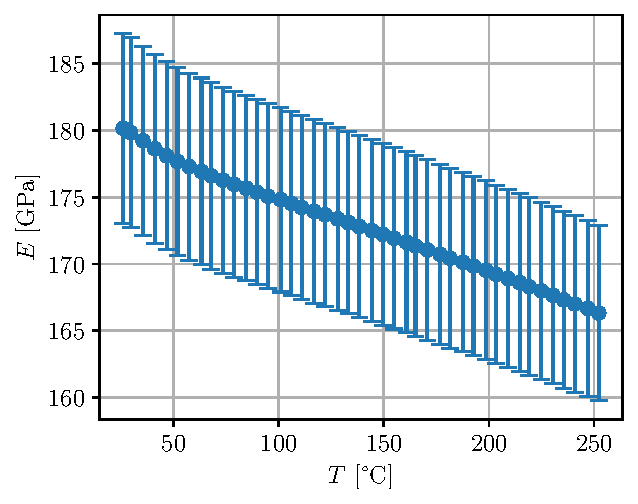
\includegraphics{figures/acier_doux_module_young_temp.pdf}
    \caption{Module de Young d'un échantillon d'acier doux en fonction de la température}
    \label{fig:module_young_temp}
\end{figure}